\documentclass[11pt]{article}

\usepackage[review]{acl}

\usepackage{times}
\usepackage{latexsym}
\usepackage[T1]{fontenc}
\usepackage[utf8]{inputenc}
\usepackage{microtype}
\usepackage{inconsolata}
\usepackage{graphicx}
\usepackage{amsmath}
\usepackage{booktabs}
\usepackage{url}

\title{LSR Interactive: An Educational Tool for Exploring\\Density Collapse in Embedding-Based Retrieval}

\author{Alison Cossette \\
  Independent Researcher \\
  \texttt{alison@claritrace.com}}

\begin{document}
\maketitle

\begin{abstract}
We present \textbf{LSR Interactive}, an open-source reactive notebook built with marimo that provides hands-on exploration of \emph{density collapse}---the phenomenon where embedding-based retrieval returns redundant, low-diversity result sets despite high similarity scores. The tool implements Local Spectral Retrieval (LSR), a method that applies local PCA to threshold-defined neighborhoods to select variance-maximizing document subsets in $O(Nd)$ time. Through a gamified interface with configurable collapse severity, interactive 3D visualizations, side-by-side method comparison (LSR vs.\ top-$k$ vs.\ MMR vs.\ random), and real-time eigenvalue spectrum analysis, the system makes the geometric structure of retrieval neighborhoods tangible. Users can manipulate collapse parameters, observe how different retrieval strategies respond, and develop intuition for when diversity-aware retrieval is necessary. The tool serves both as a pedagogical resource for understanding retrieval geometry and as a diagnostic workbench for practitioners evaluating retrieval pipelines. A live demo is available online.\footnote{\url{https://molab.marimo.io/github/alisoncossette/lsr-research/blob/master/lsr_interactive.py}} Source code: \url{https://github.com/alisoncossette/lsr-research}
\end{abstract}

\section{Introduction}

Embedding-based retrieval systems---the backbone of modern retrieval-augmented generation (RAG) pipelines \citep{lewis2020rag, karpukhin2020dense}---select documents by cosine similarity to a query vector. This approach is fast and effective for factual queries with clear best passages. However, when retrieval must assemble \emph{diverse evidence}---for multi-hop reasoning \citep{yang2018hotpotqa}, exploratory search, video keyframe selection, or robotic demonstration retrieval---top-$k$ cosine retrieval fails silently by returning redundant sets drawn from collapsed embedding regions.

\emph{Density collapse} occurs when embedding models map semantically related but informationally distinct documents into tight clusters. Threshold-based retrieval amplifies this: when many near-duplicate vectors exceed the similarity cutoff, top-$k$ selection draws almost exclusively from these dense regions. The result is high similarity scores but low informational coverage.

Maximal Marginal Relevance \citep[MMR;][]{carbonell1998mmr} addresses this via iterative diversity penalization, but its $O(Nk^2d)$ cost makes it impractical at the scale where diversity matters most ($k \geq 50$, $d \geq 1536$). Local Spectral Retrieval \citep[LSR;][]{cossette2026lsr} fills this gap by applying PCA to the local neighborhood and sampling along principal directions in $O(Nd)$ time, achieving 31--388$\times$ speedup over MMR.

Despite the practical importance of density collapse, no existing tool lets practitioners \emph{see} it, manipulate it, or develop intuition for when it matters. We address this gap with \textbf{LSR Interactive}, a reactive notebook that makes retrieval geometry tangible through interactive visualization and gamified exploration.

\section{System Overview}

LSR Interactive is built on \textbf{marimo} \citep{marimo2024}, a reactive Python notebook framework where cell outputs automatically update when inputs change. This reactivity is essential: as users adjust collapse severity, threshold, or retrieval depth, all downstream visualizations and metrics update instantly, enabling rapid experimentation.

The system is structured as a four-chapter guided experience:

\subsection{Chapter 1: Configuring the Problem}

Users select a \emph{difficulty level} (easy through chaos) that controls three parameters of a synthetic embedding generator:

\begin{itemize}
    \item \textbf{Collapse factor} (0.3--0.99): Controls the variance ratio along the first principal component. Higher values produce more severe density collapse.
    \item \textbf{Document count} (80--200): Size of the candidate pool.
    \item \textbf{Cluster count} (2--5): Number of paraphrase clusters in the neighborhood.
\end{itemize}

Fine-grained controls allow adjusting the similarity threshold $\tau$ (0.50--0.95), retrieval depth $k$ (3--20), and random seed. All parameters use reactive UI elements; changes propagate immediately.

\subsection{Chapter 2: Visualizing the Neighborhood}

The core visualization presents the embedding neighborhood as an interactive 3D scatter plot (Figure~\ref{fig:battlefield}). Documents above the similarity threshold are colored by cluster membership; those below threshold appear as faint outlines. The query vector is rendered as a gold diamond, and the principal collapse axis is shown as an orange arrow.

A companion histogram displays the similarity distribution with the threshold line overlaid, giving users immediate feedback on how threshold choice affects neighborhood size and composition. A cluster breakdown table quantifies paraphrase distribution.

This visualization makes density collapse \emph{visible}: at high collapse factors, the 3D scatter compresses into a cigar-shaped distribution where most variance concentrates along a single direction---the geometric signature that LSR detects and exploits.

\begin{figure}[t]
    \centering
    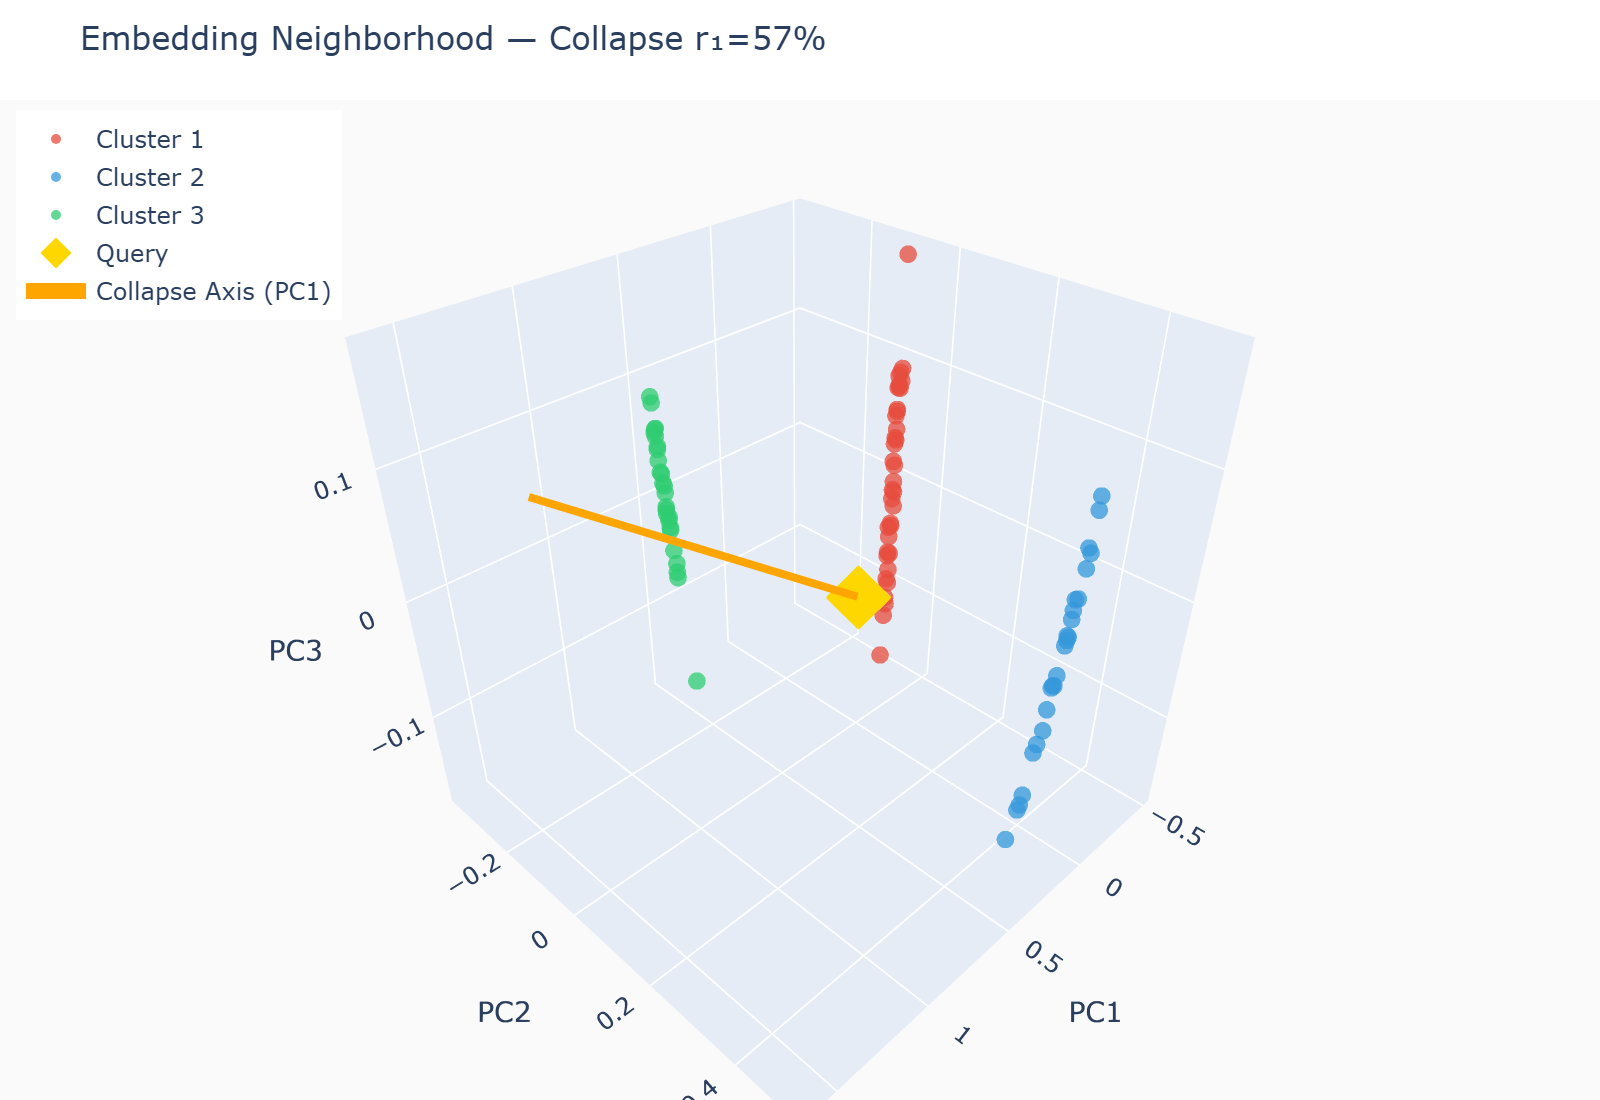
\includegraphics[width=\columnwidth]{figs/screenshot_battlefield.png}
    \caption{The ``Battlefield'' visualization: 3D embedding neighborhood with cluster coloring, query point (gold diamond), and collapse axis (orange arrow). At high collapse, the neighborhood compresses into an elongated structure along PC1.}
    \label{fig:battlefield}
\end{figure}

\subsection{Chapter 3: Method Selection}

Users select from four retrieval strategies:

\begin{enumerate}
    \item \textbf{LSR} --- PCA-based quantile sampling along the dominant principal direction. Selects documents that span the variance structure.
    \item \textbf{Top-$k$} --- Highest cosine similarity. Fast but diversity-blind.
    \item \textbf{MMR} --- Iterative relevance-diversity tradeoff. Effective but $O(Nk^2d)$.
    \item \textbf{Random} --- Uniform random sampling from the threshold neighborhood. Baseline.
\end{enumerate}

Each method includes an adaptive explanation that responds to the current data: when collapse is severe ($r_1 \geq 0.70$), LSR's description highlights that the geometry is ``perfectly suited'' for spectral sampling. When collapse is weak ($r_1 < 0.50$), it recommends falling back to MMR---demonstrating the adaptive routing logic of the full LSR framework.

\subsection{Chapter 4: Evaluation and Comparison}

\paragraph{Scoring system.} Selected documents are evaluated on a 0--100 scale across four weighted metrics:

\begin{itemize}
    \item \textbf{Redundancy} (40 pts): Average pairwise cosine similarity among selected documents (lower is better).
    \item \textbf{Cluster diversity} (15 pts): Number of distinct clusters represented.
    \item \textbf{Spatial coverage} (30 pts): Standard deviation of selected embeddings in the full-dimensional space.
    \item \textbf{Relevance} (15 pts): Mean cosine similarity to query.
\end{itemize}

Scores map to letter grades (S/A/B/C/F), providing intuitive feedback.

\paragraph{Leaderboard.} All four methods run on the same neighborhood, and results are presented in a ranked leaderboard with bar chart visualization and a detailed metrics table (Figure~\ref{fig:leaderboard}). This side-by-side comparison is the system's primary educational tool: users observe that LSR and MMR consistently outperform top-$k$ on diversity metrics in collapsed neighborhoods, that random sampling provides surprisingly good diversity (but poor relevance), and that the methods converge as collapse severity decreases.

\paragraph{Eigenvalue spectrum.} A dedicated panel displays the eigenvalue spectrum of the neighborhood's covariance matrix, with PC1 highlighted. The cumulative explained variance curve and collapse ratio $\lambda_1 / (\lambda_2 + \lambda_3)$ are shown alongside severity labels (EXTREME / HIGH / MODERATE / LOW). This connects the visual intuition from the 3D plot to the quantitative diagnostic ($r_1$) that drives LSR's adaptive routing.

\begin{figure}[t]
    \centering
    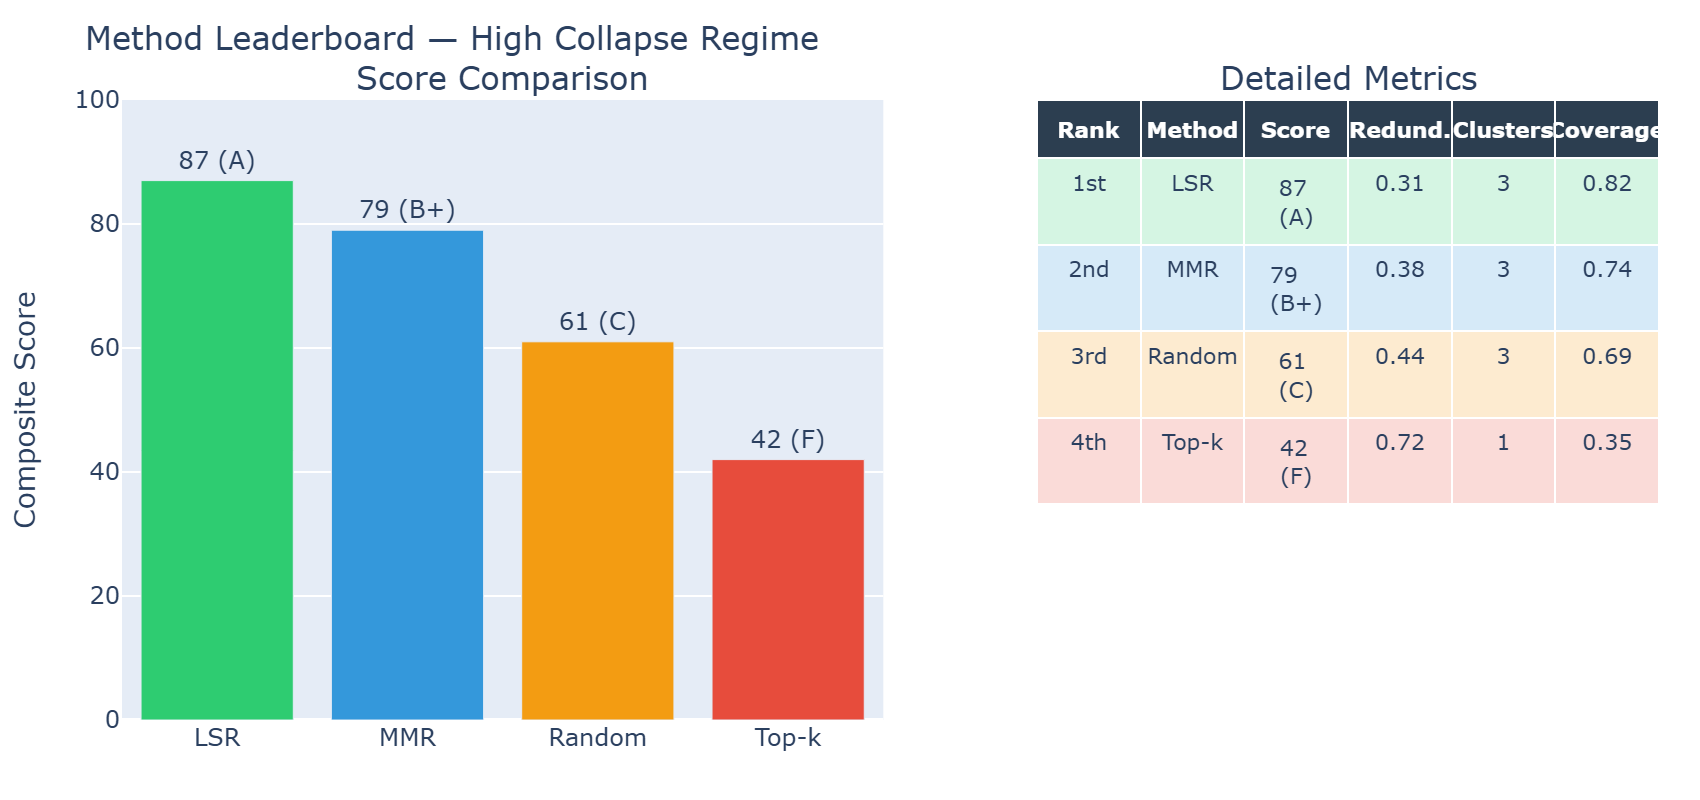
\includegraphics[width=\columnwidth]{figs/screenshot_leaderboard.png}
    \caption{The leaderboard comparison: four methods ranked by composite score. In collapsed neighborhoods, LSR and MMR substantially outperform top-$k$, while in low-collapse settings all methods converge---demonstrating when diversity-aware retrieval provides genuine benefit.}
    \label{fig:leaderboard}
\end{figure}

\paragraph{Scaling benchmark.} An optional timing comparison measures LSR vs.\ MMR across embedding dimensions from 3 to 1,024, demonstrating the computational advantage that motivates LSR: the gap widens with dimensionality, reaching orders-of-magnitude speedup at production-scale dimensions.

\section{Implementation}

\subsection{Architecture}

The system consists of three components:

\begin{enumerate}
    \item \textbf{Synthetic data generator}: Produces controllable embedding neighborhoods with tunable collapse, cluster count, and noise. Embeddings are generated in 256 dimensions with specified variance structure, then unit-normalized.
    \item \textbf{Retrieval engine}: Implements LSR (power-iteration PCA + quantile sampling), top-$k$, MMR, and random baselines. The LSR implementation uses $T = 10$ power iterations to compute the dominant eigenvector without forming the full covariance matrix.
    \item \textbf{Visualization layer}: Plotly-based interactive 3D scatter plots, histograms, bar charts, and eigenvalue spectrum displays, all integrated through marimo's reactive cell graph.
\end{enumerate}

\subsection{Reactivity Model}

marimo's dataflow-based reactivity ensures consistency: when a user changes the collapse factor, the entire downstream pipeline---data generation, retrieval, scoring, and visualization---re-executes automatically. This eliminates the stale-state bugs common in traditional Jupyter notebooks and enables fluid experimentation.

\subsection{Dependencies and Installation}

The system requires Python $\geq$ 3.11 and four packages: \texttt{marimo}, \texttt{numpy}, \texttt{scikit-learn}, and \texttt{plotly}. Dependencies are specified via PEP 723 inline metadata, enabling single-command execution:

\begin{verbatim}
  marimo run lsr_interactive.py
\end{verbatim}

No external APIs, databases, or GPU hardware are required. The full LSR library (\texttt{pip install lsr-retrieval}) is also available for integration into production pipelines.

\section{Use Cases}

\subsection{Pedagogy}
The gamified framing (``The Diversity Quest: Can You Beat the Algorithm?'') is designed for classroom and tutorial settings. Students adjust collapse severity and observe how retrieval strategies respond, building geometric intuition for high-dimensional retrieval that textbook descriptions of cosine similarity cannot provide. The letter-grade scoring system provides immediate, interpretable feedback.

\subsection{Practitioner Diagnostics}
For practitioners evaluating whether their retrieval pipeline suffers from density collapse, the tool provides a mental model: by matching the synthetic collapse patterns to their production data characteristics, practitioners can estimate whether diversity-aware retrieval would improve their system and which method (LSR vs.\ MMR) is appropriate given their latency budget.

\subsection{Research Prototyping}
The modular architecture makes it straightforward to add new retrieval methods for comparison. Researchers developing alternative diversity strategies can implement a selection function and immediately visualize its behavior alongside LSR, MMR, and baselines across controlled collapse regimes.

\section{Related Systems}

Several tools address related aspects of retrieval visualization. \textbf{Embedding Projector} \citep{smilkov2016embedding} provides t-SNE/UMAP visualization of embedding spaces but does not model retrieval or diversity. \textbf{LangChain} and \textbf{LlamaIndex} provide retrieval pipeline tooling but no interactive geometric visualization. \textbf{BEIR} benchmarks retrieval quality across datasets but focuses on aggregate metrics rather than per-query geometric structure.

LSR Interactive is, to our knowledge, the first tool that combines (a) controllable synthetic collapse, (b) interactive 3D neighborhood visualization, (c) side-by-side multi-method comparison, and (d) real-time eigenvalue diagnostics in a single reactive interface.

\section{Conclusion}

LSR Interactive makes density collapse---an abstract geometric concept---tangible through interactive visualization and gamified exploration. By enabling users to see how retrieval strategies respond to different collapse geometries, the tool bridges the gap between theoretical understanding and practical intuition. The reactive marimo framework ensures that exploration is fluid and state is always consistent. We release the tool as open-source software to support teaching, research, and practitioner adoption of diversity-aware retrieval methods.

\section*{Limitations}

The current implementation uses synthetic data with controllable collapse rather than production embeddings. While this enables precise control over experimental conditions, it does not capture the full complexity of real-world embedding distributions. The scoring rubric weights (40/15/30/15) reflect our judgment about metric importance but are not empirically calibrated. The 3D visualization projects 256-dimensional data to three dimensions, which may obscure structure visible only in higher dimensions.

\section*{Ethics Statement}

This tool is designed for educational and research purposes. The synthetic data generator does not use or produce any personal, sensitive, or copyrighted content. The retrieval methods implemented are general-purpose and do not encode demographic or content-based biases beyond those inherited from the embedding model used at deployment time.

\bibliography{refs}

\end{document}
